\section{PHƯƠNG TRÌNH BẬC NHẤT HAI ẨN VÀ HỆ HAI PHƯƠNG TRÌNH BẬC NHẤT HAI ẨN} % Tên bài
\subsection{Phương trình bậc nhất hai ẩn}
\subsubsection{Kiến thức trọng tâm}
\begin{tomtat}
\begin{itemize}
	\item Phương trình bậc nhất hai ẩn $x$ và $y$ là hệ thức dạng $a x+b y=c$, trong đó $a$, $b$ và $c$ là các số đã biết, $a \neq 0$ hoặc $b \neq 0$.
	\item Mỗi cặp số $\left(x_{0}; y_{0}\right)$ được gọi là một nghiệm của phương trình nếu $a x_{0}+b y_{0}=c$.
	\item Trong mặt phẳng tọa độ, tập hợp các điểm có tọa độ $(x ; y)$ thỏa mãn phương trình bậc nhất hai ẩn $a x+b y=c$ là một đường thẳng. Đường thẳng đó gọi là đường thẳng $a x+b y=c$.
\end{itemize}
\end{tomtat}
\subsection{Hệ hai phương trình bậc nhất hai ẩn}
\subsubsection{Kiến thức trọng tâm}
\begin{tomtat}
\begin{itemize}
\item Cặp hai phương trình bậc nhất hai ẩn $a x+b y=c$ và $a' x+b' y=c'$ được gọi là một hệ hai phương trình bậc nhất hai ẩn. Ta thường viết hệ phương trình đó dưới dạng
$$
\heva{&a x+b y=c \\
	&a' x+b' y=c'
}
$$
Trong đó $a$ và $b$ và $a'$ và $b'$ không đồng thời bằng $0$.
\item Mỗi cặp số $\left(x_{0} ; y_{0}\right)$ được gọi là một nghiệm của hệ phương trình trên nếu nó đồng thời là nghiệm của cả hai phương trình của hệ.		
\end{itemize}
\end{tomtat}
\begin{dang}{Xác định phương trình bậc nhất hai ẩn và nghiệm của nó}
\end{dang}
\begin{vd}%[Dự án EX-9-Đề Cương Toán 9]%[Nguyễn Quang Hiệp]%[9D1N2-1]
	Trong các phương trình sau, phương trình nào là phương trình bậc nhất hai ẩn? Hãy giải thích lý do.
	\begin{multicols}{3}
		\begin{enumerate}
			\item $3x-5y=7$;
			\item $x+0y=2$;
			\item $4x+8=0$;
			\item $2x-3y^2=1$;
			\item $0x+6y=0$.
		\end{enumerate}
	\end{multicols}
	\loigiai{
		\begin{enumerate}
			\item Phương trình $3x-5y=7$ là phương trình bậc nhất hai ẩn vì cả hai hệ số của $x$ và $y$ đều khác $0$ và bậc của các ẩn đều là $1$.
			\item Phương trình $x+0y=2$ là phương trình bậc nhất hai ẩn vì hệ số của $x$ khác $0$, hệ số của $y$ bằng $0$, và bậc của các ẩn đều là $1$.
			\item Phương trình $4x+8=0$ có thể viết lại là $4x+0y+8=0$ nên là phương trình bậc nhất hai ẩn.
			\item Phương trình $2x-3y^2=1$ không phải là phương trình bậc nhất hai ẩn vì ẩn $y$ có bậc là $2$.
			\item Phương trình $0x+6y=0$ là phương trình bậc nhất hai ẩn vì hệ số của $y$ khác $0$, hệ số của $x$ bằng $0$, và bậc của các ẩn đều là $1$.
		\end{enumerate}
	}
\end{vd}
\begin{vd}%[Dự án EX-9-Đề Cương Toán 9]%[Nguyễn Quang Hiệp]%[9D1N2-1]
	Trong các cặp số $(3;2)$, $(4;-1)$, $(6;2)$, $(1;-1)$, $(2;1)$, cho biết cặp số nào là nghiệm của mỗi phương trình sau:
	\begin{multicols}{2}
		\begin{enumerate}
			\item $x-2y=2$;
			\item $3x+y=7$.
		\end{enumerate}
	\end{multicols}
	\loigiai{
		\begin{enumerate}
			\item Xét phương trình $x-2y=2$
		\begin{itemize}
			\item Thay giá trị $x=3$, $y=2$ vào vế trái của phương trình, ta có $3-2\cdot 2=-1\neq 2$, do đó cặp số $(3;2)$ không phải nghiệm của phương trình $x-2y=2$.\\
			\item Thay giá trị $x=4$, $y=-1$ vào vế trái, ta có $4-2\cdot(-1)=6\neq 2$, do đó cặp số $(4;-1)$ không phải nghiệm của phương trình.\\
			\item Thay giá trị $x=6$, $y=2$ vào vế trái, ta có $6-2\cdot 2=2=2$, do đó cặp số $(6;2)$ là nghiệm của phương trình.\\
			\item Thay giá trị $x=1$, $y=-1$ vào vế trái, ta có $1-2\cdot(-1)=3\neq 2$, do đó cặp số $(1;-1)$ không phải nghiệm của phương trình.\\
			\item Thay giá trị $x=2$, $y=1$ vào vế trái, ta có $2-2\cdot 1=0\neq 2$, do đó cặp số $(2;1)$ không phải nghiệm của phương trình.		
		\end{itemize}
		Vậy chỉ có cặp số $(6;2)$ là nghiệm của phương trình $x-2y=2$.
		\item Xét phương trình $3x+y=7$
		\begin{itemize}
			\item Thay giá trị $x=3$, $y=2$ vào vế trái, ta có $3\cdot 3+2=11\neq 7$, do đó cặp số $(3;2)$ không phải nghiệm của phương trình.\\
			\item Thay giá trị $x=4$, $y=-1$ vào vế trái, ta có $3\cdot 4+(-1)=11\neq 7$, do đó cặp số $(4;-1)$ không phải nghiệm của phương trình.\\
			\item Thay giá trị $x=6$, $y=2$ vào vế trái, ta có $3\cdot 6+2=20\neq 7$, do đó cặp số $(6;2)$ không phải nghiệm của phương trình.\\
			\item Thay giá trị $x=1$, $y=-1$ vào vế trái, ta có $3\cdot 1+(-1)=2\neq 7$, do đó cặp số $(1;-1)$ không phải nghiệm của phương trình.\\
			\item Thay giá trị $x=2$, $y=1$ vào vế trái, ta có $3\cdot 2+1=7$, do đó cặp số $(2;1)$ là nghiệm của phương trình của phương trình.		
			\end{itemize}
			Vậy chỉ có cặp số $(2;1)$ là nghiệm của phương trình $3x+y=7$.
		\end{enumerate}
	}
\end{vd}

\begin{vd}%[Dự án EX-9-Đề Cương Toán 9]%[Nguyễn Quang Hiệp]%[9D1N2-1]
	Giả sử $(x; y)$ là nghiệm của phương trình bậc nhất hai ẩn $2x+3y=5$. Tìm giá trị thích hợp điền vào chỗ trống trong bảng sau rồi cho biết nghiệm tổng quát của phương trình.
	\begin{center}
		\renewcommand{\arraystretch}{1.5}
       \setlength{\tabcolsep}{18pt} 
       \begin{tabular}{|l|l|l|l|l|l|}
	\hline
	$x$ &$-2$ &$-1$ & $0$ & $1$ & $2$ \\
	\hline
	$y$ & & & & & \\
	\hline
\end{tabular}
	\end{center}
	\loigiai{\begin{center}
		    \renewcommand{\arraystretch}{1.8}
		\setlength{\tabcolsep}{18pt} 
		\begin{tabular}{|l|l|l|l|l|l|}
			\hline
			$x$ &$-2$ &$-1$ & $0$ & $1$ & $2$ \\
			\hline
			$y$ &$3$ & $\dfrac{7}{3}$&$\dfrac{5}{3}$ &1 &$\dfrac{1}{3}$ \\
			\hline
		\end{tabular}
		\end{center}
		Rút ra $y=\dfrac{5-2 x}{3}$. Tìm được nghiệm $\left(x ; \dfrac{5-2 x}{3}\right)$ với $x \in \mathbb{R}$ tùy ý.
	}
\end{vd}
\begin{vd}%[Dự án EX-9-Đề Cương Toán 9]%[Nguyễn Quang Hiệp]%[9D1H2-1]
	Cho phương trình $2x+m y=0$ với $m$ là một hằng số cho trước.
	\begin{enumerate}
		\item Phương trình trên có phải là phương trình bậc nhất hai ẩn không?
		\item Tìm điều kiện của $m$ để phương trình nhận cặp số $(3;1)$ là nghiệm.
	\end{enumerate}
	\loigiai{
		\begin{enumerate}
			\item Phương trình $2x+my=0$ là phương trình bậc nhất hai ẩn, vì hệ số của $x$ là $2\neq 0$ và $m$ là tham số bất kỳ.
			\item Thay $x=3$, $y=1$ vào phương trình, ta có
			\allowdisplaybreaks
			\begin{eqnarray*}
				2\cdot 3 + m\cdot 1 &=& 0 \\
				6 + m &=& 0 \\
				m &=& -6
			\end{eqnarray*}
			Vậy để phương trình nhận cặp số $(3;1)$ là nghiệm thì $m = -6$.
		\end{enumerate}
	}
\end{vd}
\begin{vd}%[Dự án EX-9-Đề Cương Toán 9]%[Nguyễn Quang Hiệp]%[9D1H2-1]
	Tìm tất cả các giá trị của tham số $m$ để cặp số $(2;-1)$ là nghiệm của phương trình $m x-5y=3m-1$.
	\loigiai{
		Thay $x=2$, $y=-1$ vào phương trình, ta được
		   \allowdisplaybreaks
		\begin{eqnarray*}
			m\cdot 2 - 5\cdot(-1) &=& 3m - 1 \\
			2m + 5 &=& 3m - 1 \\
			2m - 3m &=& -1 - 5 \\
			-m &=& -6 \\
			m &=& 6.
		\end{eqnarray*}
		Vậy với $m=6$ thì cặp số $(2;-1)$ là nghiệm của phương trình đã cho.
	}
\end{vd}

\begin{dang}{Biểu diễn hình học các nghiệm của phương trình bậc nhất 2 ẩn}
	\textbf{Phương pháp giải:} Để biểu diễn tất cả các nghiệm của phương trình bậc nhất hai ẩn $a x+b y=c$ trên hệ trục tọa độ, ta thực hiện các bước sau:\\
	Bước $1$. Tìm hai nghiệm của phương trình $\left(x_{1}; y_{1}\right)$ và $\left(x_{2}; y_{2}\right)$;\\
	Bước $2$. Biểu diễn hai điểm có tọa độ là hai nghiệm vừa tìm được trên mặt phẳng tọa độ, rồi vẽ đường thẳng đi qua hai điểm đó.
\end{dang}
\begin{vd}%[Dự án EX-9-Đề Cương Toán 9]%[Nguyễn Quang Hiệp]%[9D1H2-1]
	Cho phương trình bậc nhất hai ẩn $3x-y=1$.
	\begin{enumerate}
		\item Chứng tỏ rằng các cặp số $(1; 2),(0;-1),(2; 5)$ là các nghiệm của phương trình trên;
		\item Trong mặt phẳng tọa độ $Oxy$, hãy biểu diễn các nghiệm $(1; 2),(0;-1),(2; 5)$ của phương trình trên.
	\end{enumerate}
	\loigiai{\begin{enumerate}
			\item Xét các cặp số $(1; 2),(0 ;-1),(2 ; 5)$ :
			\begin{itemize}
				\item Thay giá trị $x=1$ và $y=2$ vào vế trái của phương trình ta có $3\cdot 1-2=1$, do đó cặp số $(1; 2)$ là nghiệm của phương trình $3 x-y=1$;
				\item Thay giá trị $x=0$ và $y=-1$ vào vế trái của phương trình ta có $3\cdot 0-(-1)=1$, do đó cặp số $(0 ;-1)$ là nghiệm của phương trình $3 x-y=1$. 
				\item Thay giá trị $x=2$ và $y=5$ vào vế trái của phương trình ta có $3\cdot 2-5=1$, do đó cặp số $(2; 5)$ là nghiệm của phương trình $3 x-y=1$.
			\end{itemize}
			\item \begin{center}
				\begin{tikzpicture}[line join=round, line cap=round,>=stealth,thick]
					\tikzset{every node/.style={scale=0.9}}
					\draw[->] (-2,0)--(4.5,0) node[above] {$x$};
					\draw[->] (0,-2.1)--(0,5.5) node[below left] {$y$};
					\draw (0,0) node [below left] {$O$};
					\foreach \x/\nx in {1/1,2/2,3/3,4/4,-1/-1}
					\draw[thin] (\x,1pt)--(\x,-1pt) node [below] {$\nx$};
					\foreach \y/\ny in {1/1,2/2,3/3,4/4,-1/-1}
					\draw[thin] (1pt,\y)--(-1pt,\y) node [left] {$\ny$};
					\draw[dashed,thin](1,0)--(1,2) circle(1pt)  node [right,scale=.75] {$A\left( 1;2\right) $}--(0,2) ;
					\draw[dashed,thin](2,0)--(2,5) circle(1pt) node [right,scale=.75] {$B\left( 2;5\right) $}--(0,5);
					\draw[dashed,thin](0,0)--(0,-1) circle(1pt) node [right,scale=.75] {$C\left( 0;-1\right) $};
					\begin{scope}
						\clip (-2,-2) rectangle (5,5.5);
						\draw[samples=200,domain=-5:5,smooth,variable=\x] plot (\x,{3*(\x)+-1});
					\end{scope}
				\end{tikzpicture} 
			\end{center}
		\end{enumerate}
	}
\end{vd}
\begin{vd}%[Dự án EX-9-Đề Cương Toán 9]%[Nguyễn Quang Hiệp]%[9D1H2-1]
	Viết nghiệm và biểu diễn hình học tất cả các nghiệm của mỗi phương trình bậc nhất hai ẩn sau:
\begin{multicols}{3}
		\begin{enumerate}
		\item $x+2y=3$;
		\item $0x+3y=6$;
		\item $x-y=1$.
	\end{enumerate}
\end{multicols}
	\loigiai{\begin{enumerate}
			\item $x+2y=3$ suy ra $y=\dfrac{-x+3}{2}$.\\			
			Vậy nghiệm của phương trình là $\left(x ; \dfrac{-x+3}{2}\right)$ với $x \in \mathbb{R}$ tùy ý.\\
			Chọn $x=3$ suy ra $y=0$. Ta có điểm $A(3 ; 0)$;\\
			Chọn $x=1$ suy ra $y=1$. Ta có điểm $B(1; 1)$.
			\begin{center}
			\begin{tikzpicture}[>=stealth,line join=round,line cap=round,font=\footnotesize,scale=1]
				\tikzset{declare function={
						x1=-2.2;x2=4.5;y1=-1.5;y2=3.5;
						a=-1/2;b=3/2;
						f(\x)=a*(\x)+b;
				}}
				\begin{scope}
					\clip (x1,y1)rectangle(x2,y2);
					\draw [smooth,samples=100,domain=x1:x2]plot(\x,{f(\x)});
				\end{scope}
				\draw[->] (0,y1)--(0,y2)node[left]{$y$};
				\draw[->] (x1,0)--(x2,0)node[above]{$x$};
				\filldraw(0,0)circle(1.2pt)node[below left]{$O$};
				\foreach \x/\goc in {1/-90,2/-90,3/-90}{
					\draw[fill=black] (\x,0)circle(1.2pt) node[shift={(\goc:2.8mm)}]{$\x$};
				}
				\foreach \y/\goc in {1/180,2/180,3/180}{
					\draw[fill=black] (0,\y)circle(1.2pt)node[shift={(\goc:2.8mm)}]{$\y$};
				}
				\draw[dashed](0,1)-|(1,0);
					\path (1,1)coordinate (A);
				\foreach \point/\goc in {A/90}{
					\draw[fill=black](\point)circle(1.2pt)+(\goc:2mm)node[scale=.8]{};
				}
			\end{tikzpicture}
			\end{center}
			\item $0 x+3 y=6$ suy ra $y=2$;\\
			Vậy nghiệm của phương trình là $(x ; 2)$ với $x \in \mathbb{R}$ tùy ý.\\
			Chọn $x=0$ suy ra $y=2$. Ta có điểm $A(0 ; 2)$;\\
			Chọn $x=3$ suy ra $y=2$. Ta có điểm $B(3 ; 2)$.
			\begin{center}
				\begin{tikzpicture}[>=stealth,line join=round,line cap=round,font=\footnotesize,scale=1]
					\tikzset{declare function={
							x1=-2.2;x2=4.5;y1=-1.5;y2=3.5;
							a=0;b=2;
							f(\x)=a*(\x)+b;
					}}
					\begin{scope}
						\clip (x1,y1)rectangle(x2,y2);
						\draw [smooth,samples=100,domain=x1:x2]plot(\x,{f(\x)});
					\end{scope}
					\draw[->] (0,y1)--(0,y2)node[left]{$y$};
					\draw[->] (x1,0)--(x2,0)node[above]{$x$};
					\filldraw(0,0)circle(1.2pt)node[below left]{$O$};
					\foreach \x/\goc in {1/-90,2/-90,3/-90}{
						\draw[fill=black] (\x,0)circle(1.2pt) node[shift={(\goc:2.8mm)}]{$\x$};
					}
					\foreach \y/\goc in {1/180,2/145,3/180}{
						\draw[fill=black] (0,\y)circle(1.2pt)node[shift={(\goc:2.8mm)}]{$\y$};
					}
					\draw[dashed](0,2)-|(3,0);
					\path (3,2)coordinate (A);
				\foreach \point/\goc in {A/90}{
					\draw[fill=black](\point)circle(1.2pt)+(\goc:2mm)node[scale=.8]{};
				}
				\end{tikzpicture}
			\end{center}
			\item $x-y=1$, suy ra $y=x-1$.\\
			Vậy nghiệm của phương trình là $(x ; x-1)$ với $x \in \mathbb{R}$ tùy ý.\\
			Chọn $x=1$ suy ra $y=0$. Ta có điểm $A(1; 0)$;\\
			Chọn $x=3$ suy ra $y=2$. Ta có điểm $B(3 ; 2)$.
			\begin{center}
			\begin{tikzpicture}[>=stealth,line join=round,line cap=round,font=\footnotesize,scale=1]
				\tikzset{declare function={
						x1=-2.2;x2=4.5;y1=-2.5;y2=3.5;
						a=1;b=-1;
						f(\x)=a*(\x)+b;
				}}
				\begin{scope}
					\clip (x1,y1)rectangle(x2,y2);
					\draw [smooth,samples=100,domain=x1:x2]plot(\x,{f(\x)});
				\end{scope}
				\draw[->] (0,y1)--(0,y2)node[left]{$y$};
				\draw[->] (x1,0)--(x2,0)node[above]{$x$};
				\filldraw(0,0)circle(1.2pt)node[below left]{$O$};
				\foreach \x/\goc in {1/-90,2/-90,3/-90}{
					\draw[fill=black] (\x,0)circle(1.2pt) node[shift={(\goc:2.8mm)}]{$\x$};
				}
				\foreach \y/\goc in {1/180,2/180,3/180}{
					\draw[fill=black] (0,\y)circle(1.2pt)node[shift={(\goc:2.8mm)}]{$\y$};
				}
				\draw[dashed](0,2)-|(3,0);
					\path (3,2)coordinate (A);
				\foreach \point/\goc in {A/90}{
					\draw[fill=black](\point)circle(1.2pt)+(\goc:2mm)node[scale=.8]{};
				}
			\end{tikzpicture}
			\end{center}
		\end{enumerate}
	}
\end{vd}
\begin{dang}{Xác định nghiệm của hệ phương trình bậc nhất hai ẩn}
\end{dang}
\begin{vd}%[Dự án EX-9-Đề Cương Toán 9]%[Nguyễn Quang Hiệp]%[9D1N2-2]
	Cho hệ phương trình $\heva{&2x - y = 1 \\ &x + 3y = 7}$. Trong các cặp số sau, cặp số nào là nghiệm của hệ phương trình đã cho?
	\begin{multicols}{2}
		\begin{enumerate}
		\item $(2;1)$;
		\item $(1;2)$.
	\end{enumerate}
	\end{multicols}
	\loigiai{
		\begin{enumerate}
			\item Xét cặp số $(2;1)$\\
			Thay $x=2$, $y=1$ vào phương trình thứ nhất: $2\cdot 2 - 1 = 4 - 1 = 3 \neq 1$.\\
			Như vậy $(2;1)$ không phải nghiệm của hệ phương trình.
			\item Xét cặp số $(1;2)$\\
			Thay $x=1$, $y=2$ vào phương trình thứ nhất: $2\cdot 1 - 2 = 2 - 2 = 0 \neq 1$.\\
			Như vậy $(1;2)$ cũng không phải nghiệm của hệ phương trình.
		\end{enumerate}
	}
\end{vd}

\begin{vd}%[Dự án EX-9-Đề Cương Toán 9]%[Nguyễn Quang Hiệp]%[9D1N2-2]
	Cho các cặp số $(1; 2)$, $(2; 1)$, $(3; 0)$, $(0; 3)$, $(4; -1)$ và hai phương trình $\heva{
		&x + 2y = 5  \quad &(1) \\
		&3x - y = 1.  \quad &(2)
	}$
	Trong các cặp số đã cho:
	\begin{enumerate}
		\item Cặp số nào là nghiệm của phương trình $(1)$?
		\item Cặp số nào là nghiệm của hệ hai phương trình gồm $(1)$ và $(2)$?
		\item Vẽ hai đường thẳng $x+2y=5$ và $3x-y=1$ trên cùng một mặt phẳng tọa độ để minh họa.
	\end{enumerate}
	\loigiai{
		\begin{enumerate}
			\item Ta thay lần lượt từng cặp số vào phương trình $x + 2y = 5$\\
			Thay $x=1$, $y=2$, ta được $1 + 2\cdot 2 = 5$ (đúng), nên $(1;2)$ là nghiệm.\\
			Thay $x=2$, $y=1$, ta được $2 + 2\cdot 1 = 4$ (không đúng), nên $(2;1)$ không là nghiệm.\\
			Thay $x=3$, $y=0$, ta được $3 + 2\cdot 0 = 3$ (không đúng), nên $(3;0)$ không là nghiệm.\\
			Thay $x=0$, $y=3$, ta được $0 + 2\cdot 3 = 6$ (không đúng), nên $(0;3)$ không là nghiệm.\\
			Thay $x=4$, $y=-1$, ta được $4 + 2\cdot(-1) = 2$ (không đúng), nên $(4;-1)$ không là nghiệm.\\
			Vậy chỉ có cặp số $(1;2)$ là nghiệm của phương trình $(1)$.
			\item Xét các cặp số vừa kiểm tra ở trên, chỉ cần xét $(1;2)$ với phương trình $(2)$\\
			Thay $x=1$, $y=2$ vào $3x-y=1$ ta có $3\cdot 1 - 2 = 1$ (đúng).\\
			Vậy $(1;2)$ là nghiệm của cả hai phương trình, tức là nghiệm của hệ.
			\item Vẽ hai đường thẳng $x+2y=5$ và $3x-y=1$
			\begin{center}
			\begin{tikzpicture}[>=stealth,line join=round,line cap=round,font=\footnotesize,scale=1]
				\tikzset{declare function={
						x1=-2.2;x2=6.5;y1=-2.5;y2=3.5;
						a=-1/2;b=5/2;
						f(\x)=a*(\x)+b;
						c=3;d=-1;
						g(\x)=c*(\x)+d;
				}}
				\begin{scope}
					\clip (x1,y1)rectangle(x2,y2);
					\draw [smooth,samples=100,domain=x1:x2]plot(\x,{f(\x)});
					\draw [smooth,samples=100,domain=x1:x2]plot(\x,{g(\x)});
				\end{scope}
				\draw[->] (0,y1)--(0,y2)node[left]{$y$};
				\draw[->] (x1,0)--(x2,0)node[above]{$x$};
				\filldraw(0,0)circle(1.2pt)node[below left]{$O$};
				\foreach \x/\goc in {1/-90,2/-90,3/-90,4/-90,5/-90}{
					\draw[fill=black] (\x,0)circle(1.2pt) node[shift={(\goc:2.8mm)}]{$\x$};
				}
				\foreach \y/\goc in {1/180,2/180,3/180}{
					\draw[fill=black] (0,\y)circle(1.2pt)node[shift={(\goc:2.8mm)}]{$\y$};
				}
				\draw[dashed](0,2)-|(1,0);
			\path (1,2)coordinate (A);
			\foreach \point/\goc in {A/90}{
				\draw[fill=black](\point)circle(1.2pt)+(\goc:2mm)node[scale=.8]{};
			}	
			\end{tikzpicture}	
			\end{center}
		\end{enumerate}
	}
\end{vd}
\begin{dang}{Một số bài toán thực tế}
\end{dang}
\begin{vd}%[Dự án EX-9-Đề Cương Toán 9]%[Nguyễn Quang Hiệp]%[9D1H2-3]
	Cô Hạnh có hai khoản đầu tư với lãi suất là $8\%$ và $10\%$ mỗi năm. Cô Hạnh thu được tiền lãi từ hai khoản đầu tư đó là $160$ triệu đồng mỗi năm. Viết phương trình bậc nhất hai ẩn cho hai khoản đầu tư của cô Hạnh và chỉ ra ba nghiệm của phương trình đó.
	\loigiai
	{ Gọi $x$ (triệu đồng) là khoản  đầu tư với lãi suất là $8\%$ mỗi năm ($x>0$). Khi đó, tiền lãi thu được mỗi năm từ khoản đầu tư này là \[8\%\cdot x=\dfrac{2x}{25}\ (\mbox{triệu đồng}).\]
		Gọi $y$ (triệu đồng) là khoản  đầu tư với lãi suất là $10\%$ mỗi năm ($y>0$). Khi đó, tiền lãi thu được mỗi năm từ khoản đầu tư này là \[10\%\cdot y=\dfrac{y}{10}\ (\mbox{triệu đồng}).\]
		Ta có phương trình bậc nhất hai ẩn $x$, $y$ cho hai khoản đầu tư của cô Hạnh là 
		\[\dfrac{2x}{25}+\dfrac{y}{10}=160\ \mbox{hay }4x+5y=8\, 000.\]
		Ba nghiệm của phương trình trên là $(100; 1\, 520), (500;1\,200),(1\, 000;800)$.
	}
\end{vd}
\begin{vd}%[Dự án EX-9-Đề Cương Toán 9]%[Nguyễn Quang Hiệp]%[9D1H2-3]
	Bác Ninh có hai khoản tiền thu được do bán bàn ăn và bàn làm việc cho công ty A. Bàn ăn giá $500\,000$ đồng/chiếc, bàn làm việc giá $700\,000$ đồng/chiếc. Bác Ninh thu được tổng số tiền $11\,200\,000$ đồng từ hai khoản tiền trên. Viết phương trình bậc nhất hai ẩn cho tổng số tiền bác Ninh thu được từ hai khoản tiền do bán bàn ăn và bàn làm việc cho công ty A và chỉ ra hai nghiệm của phương trình đó.
	\loigiai{
		Gọi $x$ (chiếc) là số bàn ăn mà bác Ninh đã bán cho công ty A với $x \in \mathbb{N}^{*}$. Khi đó, khoản tiền bác Ninh thu được do bán bàn ăn cho công ty A là $500\,000x$ (đồng).\\
		Gọi $y$ (chiếc) là số bàn làm việc mà bác Ninh đã bán cho công ty $A$ với $y \in \mathbb{N}^{*}$. Khi đó, khoản tiền bác Ninh thu được do bán bàn làm việc cho công ty A là $700\,000y$ (đồng).\\
		Ta có phương trình bậc nhất hai ẩn cho tổng số tiền bác Ninh thu được từ hai khoản tiền do bán bàn ăn và bàn làm việc cho công ty $A$ là 
		\[500\,000x+700\,000y=11\,200\,000 \text { hay } 5 x+7 y=112.\]
		Hai nghiệm của phương trình trên là $(7; 11)$, $(14; 6)$.
	}
\end{vd}
\begin{vd}%[Dự án EX-9-Đề Cương Toán 9]%[Nguyễn Quang Hiệp]%[9D1H2-3]
	Hai bạn Dũng, Huy vào mua siêu thị mua vở và bút bi để ủng hộ các bạn học sinh vùng lũ lụt. Bạn Dũng mua $5$ quyển vở và $3$ chiếc bút bi với tổng số tiền phải trả là $39\, 000$ đồng. Bạn Huy mua $6$ quyển vở và $2$ chiếc bút bi với tổng số tiền phải trả là $42\, 000$ đồng. Giả sử giá của mỗi quyển vở là $x$ đồng $(x>0)$, giá của mỗi chiếc bút bi là $y$ đồng $(y>0)$.
	\begin{enumerate}
		\item Viết hai phương trình bậc nhất hai ẩn $x$, $y$ lần lượt biểu thị tổng số tiền phải trả của bạn Dũng, bạn Huy.
		\item Cặp số $(x;y)=(6\, 000;3\, 000)$ có phải là nghiệm của từng phương trình bậc nhất đó hay không? Vì sao?
	\end{enumerate}
	\loigiai{\begin{enumerate}
			\item Hai phương trình tương ứng là $5x+3y=39\, 000$ và $6x+2y=42\, 000$.
			\item  Vì $x$, $y$ đồng thời thỏa mãn cả hai phương trình nói trên nên ta nói \\ cặp $(x;y)=(6\, 000;3\, 000)$ là nghiệm của hệ phương trình \[\heva{& 5x+3y=39\, 000 \\ & 6x+2y=42\, 000.}\]
	\end{enumerate}}
\end{vd}
\begin{vd}%[Dự án EX-9-Đề Cương Toán 9]%[Nguyễn Quang Hiệp]%[9D1H2-3]
	Hai trường $A$ và $B$ có tổng cộng 180 học sinh tham gia ngày hội STEM. Biết rằng $15\%$ học sinh trường $A$ tham gia và $10\%$ học sinh trường $B$ tham gia đạt giải. Tổng số học sinh hai trường $A$ và $B$ đạt giải là $22$ học sinh. Gọi $x$ và $y$ lần lượt là số học sinh của trường $A$ và trường $B$ tham gia ngày hội đó.
	\begin{enumerate}
		\item Viết hệ hai phương trình bậc nhất hai ẩn $x$, $y$ biểu thị mối quan hệ giữa các đại lượng.
		\item Cặp số $(80; 100)$ có phải là nghiệm của hệ phương trình ở trên hay không? Vì sao?
	\end{enumerate}
	\loigiai{
		\begin{enumerate}
			\item 
			\begin{itemize}
				\item Số học sinh trường $A$ đạt giải là $15\% \cdot x=\dfrac{3}{20} x$;
				\item Số học sinh trường $B$ đạt giải là $10\% \cdot y=\dfrac{1}{10} y$.
				\item Tổng số học sinh hai trường $A$ và $B$ đạt giải là $\dfrac{3}{20} x+\dfrac{1}{10} y$.
				\item Do hai trường $A$ và $B$ có tổng cộng $180$ học sinh tham gia ngày hội STEM và tổng số học sinh hai trường $A$ và $B$ đạt giải là $22$ học sinh nên ta có hệ hai phương trình bậc nhất hai ẩn $x, y$ biểu thị mối quan hệ giữa các đại lượng là
				\[\heva{&x+y=180\\
					&\dfrac{3}{20} x+\dfrac{1}{10} y=22.}\]
			\end{itemize}			
			\item Thay $x=80, y=100$ vào mỗi phương trình trong hệ phương trình ở trên, ta có
			\[80+100=180; \quad \dfrac{3}{20} \cdot 80+\dfrac{1}{10} \cdot 100=22.\]
			Vậy cặp số $(80; 100)$ là nghiệm của hệ phương trình ở trên.
		\end{enumerate}
	}
\end{vd}
\subsubsection{Bài tập}
\begin{bt}%[Dự án EX-9-Đề Cương Toán 9]%[Nguyễn Quang Hiệp]%[9D1N2-1]
	Chỉ ra các phương trình bậc nhất hai ẩn $x$ và $y$ trong các phương trình sau
	\begin{multicols}{2}
	\begin{enumerate}
		\item $5y-x=-2$;
		\item $3x^2-10y=1$;
		\item $\dfrac{x^2}{x+1}-y=0$;
		\item $x+0y=4$.
	\end{enumerate}
	\end{multicols}
	\loigiai{
		Các phương trình bậc nhất hai ẩn $x$ và $y$ là $5y-x=-2$ và $x+0y=4$.
	}
\end{bt}
	\begin{bt}%[Dự án EX-9-Đề Cương Toán 9]%[Nguyễn Quang Hiệp]%[9D1N2-1]
	Giả sử $(x; y)$ là nghiệm của phương trình bậc nhất hai ẩn $2x+y=4$. Tìm giá trị thích hợp điền vào chỗ trống trong bảng sau rồi cho biết nghiệm tổng quát của phương trình.
	\begin{center}
		\begin{tabular}{|l|l|l|l|l|l|}
			\hline
			$x$ &$-2$ &$-1$ & 0 & 1 & 2 \\
			\hline
			$y$ & & & & & \\
			\hline
		\end{tabular}
	\end{center}
	\loigiai{
		Nghiệm của phương trình là $(x ;-2 x+4)$ với $x \in \mathbb{R}$ tùy ý.\\
		\begin{center}
			\begin{tabular}{|l|l|l|l|l|l|}
				\hline
				$x$ &$-2$ &$-1$ & $0$ & $1$ & $2$ \\
				\hline
				$y$ &$8$ & $6$&$4$ &$2$ &$0$ \\
				\hline
			\end{tabular}
		\end{center}
	}
\end{bt}
\begin{bt}%[Dự án EX-9-Đề Cương Toán 9]%[Nguyễn Quang Hiệp]%[9D1N2-1]
	Tìm bốn nghiệm của phương trình $3x-4y=5$.
	\loigiai 
	{
		Vì $3\cdot (-5)-4\cdot (-5)=5$ nên cặp số $(-5;-5)$ là một một nghiệm của phương trình $3x-4y=5$.\\
		Vì $3\cdot 3-4\cdot 1=5$ nên cặp số $(3;1)$ là một nghiệm của phương trình $3x-4y=5$.\\
		Vì $3\cdot (-1)-4\cdot (-2)=5$ nên cặp số $(-1;-2)$ là một nghiệm của phương trình $3x-4y=5$.\\
		Vì $3\cdot 7-4\cdot 4=5$ nên cặp số $(7;4)$ là một nghiệm của phương trình $3x-4y=5$.
	}
\end{bt}
\begin{bt}%[Dự án EX-9-Đề Cương Toán 9]%[Nguyễn Quang Hiệp]%[9D1H2-1]
	Trong mặt phẳng tọa độ $Oxy$, hãy biểu diễn các nghiệm của mỗi phương trình sau
	\begin{multicols}{2}
		\begin{enumerate}
			\item $2x-y=-1$;
			\item $-4x+0y=12$.
		\end{enumerate}
	\end{multicols}
	\loigiai{
		\begin{enumerate}
			\item Xét phương trình $2x-y=-1$. (1)
			\immini
			{
				Chuyển vế, ta có $y=2x+1$.\\
				Nếu cho $x$ một giá trị bất kì thì cặp số $(x;y)$, trong đó $y=2x+1$, là một nghiệm của phương trình (1).\\
				Do đó phương trình (1) có các nghiệm là $\heva{& x \in \mathbb{R} \\& y=2x+1.}$\\
				Trong mặt phẳng toạ độ $Oxy$, tập hợp các điểm biểu diễn các nghiệm của phương trình (1) là đường thẳng $y=2x+1$.
			}
			{
				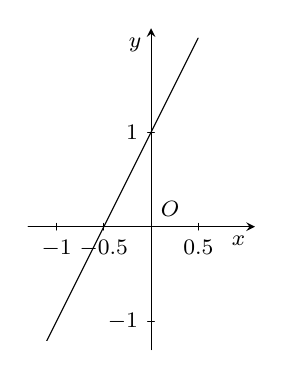
\begin{tikzpicture}[scale=1.2, font=\footnotesize, line join=round, line cap=round, >=stealth]
					\draw[->] (-1.3,0)--(1.1,0) node[below left] {$x$};
					\draw[->] (0,-1.3)--(0,2.1) node[below left] {$y$};
					\draw (0,0) node [above right] {$O$};
					\foreach \x/\nx in {-1/-1,-0.5/-0.5,0.5/0.5}
					\draw[thin] (\x,1pt)--(\x,-1pt) node [below] {$\nx$};
					\foreach \y/\ny in {-1/-1,1/1}
					\draw[thin] (1pt,\y)--(-1pt,\y) node [left] {$\ny$};
					\begin{scope}
						\clip (-1.2,-1.2) rectangle (1,2);
						\draw[samples=200,domain=-1.5:0.5,smooth,variable=\x] plot (\x,{2*(\x)+1});
					\end{scope}
				\end{tikzpicture}
			}
		
			\item Xét phương trình $-4x+0y=12$. (2)
			\immini
			{
				Chuyển vế, ta có $-4x=12$ hay $x=-3$.\\
				Nếu cho $x$ một giá trị bất kì thì cặp số $(x;y)$, trong đó $x=-3$, là một nghiệm của phương trình (3).\\
				Do đó phương trình (3) có các nghiệm là $\heva{& x =-3 \\& y\in \mathbb{R}.}$\\
				Trong mặt phẳng toạ độ $Oxy$, tập hợp các điểm biểu diễn các nghiệm của phương trình (1) là đường thẳng đi qua điểm $B(-3;0)$ và song song với trục tung (ta gọi đường thẳng này là đường thẳng $x=-3$).
			}
			{
				\begin{tikzpicture}[scale=0.75, font=\footnotesize, line join=round, line cap=round, >=stealth]
					\draw[->] (-4,0)--(1.5,0) node[below left] {$x$};
					\draw[->] (0,-2.6)--(0,3.5) node[below left] {$y$};
					\draw (0,0) node [above right] {$O$};
					\foreach \x/\nx in {-3/-3,-2/-2,-1/-1,1/1}
					\draw[thin] (\x,1pt)--(\x,-1pt) node [below left] {$\nx$};
					\foreach \y/\ny in {-1/-1,-2/-2,2/2,1/1}
					\draw[thin] (1pt,\y)--(-1pt,\y) node [left] {$\ny$};
					\draw (-3,-2.5)--(-3,3);
				\end{tikzpicture}
			}
		\end{enumerate}
	}
\end{bt}
\begin{bt}%[Dự án EX-9-Đề Cương Toán 9]%[Nguyễn Quang Hiệp]%[9D1N2-2]
	Cho hệ phương trình $\heva{&3x+y=5\\&4x+2y=8}$. Trong các cặp số sau, cặp số nào là nghiệm của hệ phương trình đã cho?
\begin{multicols}{2}
		\begin{enumerate}
		\item $(1; 2)$;
		\item $(2;-1)$.
	\end{enumerate}
\end{multicols}
	\loigiai{\begin{enumerate}
			\item Thay $x=1, y=2$ vào phương trình của hệ ta có\\
			$3\cdot 1+1\cdot 2=5  ; 4\cdot 1+2\cdot2=8 $. \\
			Suy ra cặp số $(1; 2)$ là nghiệm của hệ phương trình đã cho.
			\item Thay $x=2, y=-1$ vào phương trình của hệ ta có\\
			$3\cdot 2+1\cdot -1=5  ; 4\cdot 2+2\cdot -1=6 \neq 8 $. \\
			Suy ra cặp số $(1; 2)$ là không nghiệm của hệ phương trình đã cho.
	\end{enumerate}}
\end{bt}
\begin{bt}%[Dự án EX-9-Đề Cương Toán 9]%[Nguyễn Quang Hiệp]%[9D1H2-2]
	Cho các cặp số $(1; 2),(2; 4),(3; 7),(-1;-2),(-2;-5)$ và hệ hai phương trình $$\heva{
		&2x-y=0 \qquad\left(1\right)\\
		&3x+2y=14 \quad\left(2\right).
	}$$ Trong các cặp số đã cho
	\begin{enumerate}
		\item Cặp số nào là nghiệm của phương trình $(1)$?
		\item Cặp số nào là nghiệm của hệ hai phương trình gồm $(1)$ và $(2)$?
		\item Vẽ hai đường thẳng $2x-y=0$ và $3x+2y=14$ trên cùng một mặt phẳng tọa độ để minh họa kết luận ở câu b).
	\end{enumerate}
	\loigiai{
		\begin{enumerate}
			\item Cặp số $(1; 2) ;(2 ; 4) ;(-1;-2)$ là nghiệm của phương trình $2 x-y=0$; Cặp số $(3 ; 7) ;(-2 ; 5)$ không phải nghiệm của phương trình $2 x-y=0$;
			\item Cặp số $(2 ; 4)$ là nghiệm của cả hai phương trình $(1)$ và $(2)$.
			\item \qquad
			\begin{center}
				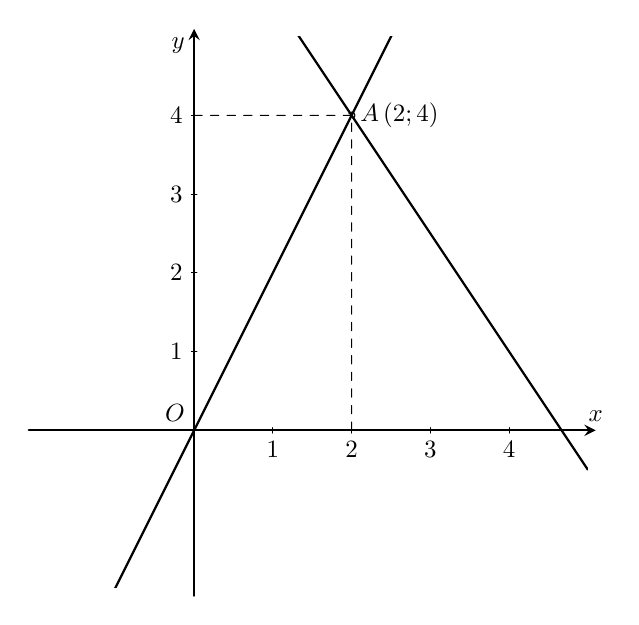
\begin{tikzpicture}[line join=round, line cap=round,>=stealth,thick]
					\tikzset{every node/.style={scale=0.9}}
					\draw[->] (-2.1,0)--(5.1,0) node[above] {$x$};
					\draw[->] (0,-2.1)--(0,5.1) node[below left] {$y$};
					\draw (0,0) node [above left] {$O$};
					\foreach \x/\nx in {1/1,2/2,3/3,4/4}
					\draw[thin] (\x,1pt)--(\x,-1pt) node [below] {$\nx$};
					\foreach \y/\ny in {1/1,2/2,3/3,4/4}
					\draw[thin] (1pt,\y)--(-1pt,\y) node [left] {$\ny$};
					\draw[dashed,thin](2,0)--(2,4)circle(1.2pt) node [right] {$A\left( 2;4\right) $} --(0,4);
					\begin{scope}
						\clip (-2,-2) rectangle (5,5);
						\draw[samples=200,domain=-5:5,smooth,variable=\x] plot (\x,{-3/2*(\x)+14/2});
						\draw[samples=200,domain=-5:5,smooth,variable=\x] plot (\x,{2*(\x)+0});
					\end{scope}
					
				\end{tikzpicture}
			\end{center}
		\end{enumerate}			
	}
\end{bt}
\begin{bt}%[Dự án EX-9-Đề Cương Toán 9]%[Nguyễn Quang Hiệp]%[9D1H2-1]
	Cho phương trình $(m-1) x+m y=12$ với $m$ là tham số.
	\begin{enumerate}
		\item Chứng tỏ rằng phương trình đã cho luôn là phương trình bậc nhất hai ẩn với mọi giá trị của $m$.
		\item Tìm giá trị của tham số $m$ để cặp số $(2; 5)$ là nghiệm của phương trình đã cho.
	\end{enumerate}
	\loigiai{
		\begin{enumerate}
			\item Ta xét các trường hợp sau:
			
			TH1: Nếu $m-1=0$, tức là $m=1$, thì phương trình trở thành $0\cdot x+y=12$. Đây là phương trình bậc nhất hai ẩn.\\
			TH2: Nếu $m=0$, thì phương trình trở thành $-1x+0\cdot y=12$. Đây là phương trình bậc nhất hai ẩn.\\
			TH3: Nếu $m \neq 0, m \neq 1$, thì hệ số của cả $x$ và $y$ đều khác $0$. Khi đó phương trình đã cho là phương trình bậc nhất hai ẩn.\\
			Vậy phương trình đã cho luôn là phương trình bậc nhất hai ẩn với mọi giá trị của $m$.
			\item Thay giá trị $x=2$ và $y=5$ và phương trình đã cho ta có $(m-1) \cdot 2+m \cdot 5=12$, suy ra $2m-2+5m=12$.\\
			Khi đó $7m=14$, tức là $m=2$.\\
			Vậy để cặp số $(2; 5)$ là nghiệm của phương trình đã cho thì $m=2$.
		\end{enumerate}
	}
\end{bt}

\begin{bt}%[Dự án EX-9-Đề Cương Toán 9]%[Nguyễn Quang Hiệp]%[9D1H2-3]
	Ba bạn An, Bình, Chi cùng đi nhà sách. Cả ba bạn đã mua hết $279\,000$ đồng. Ba bạn đã mua $3$ quyển truyện với giá $45\,000$ đồng/quyển và mua thêm bút bi, bút chì màu. Giá của bút bi và bút chì màu lần lượt là $3\,600$ đồng/chiếc và $5\,000$ đồng/chiếc. Gọi $x$ và $y$ lần lượt là số chiếc bút bi và bút chì màu mà ba bạn đã mua. Viết phương trình bậc nhất hai ẩn cho số tiền mà ba bạn đã dùng để mua bút bi, bút chì màu và chỉ ra một nghiệm của phương trình đó.
	\loigiai{
		Số tiền ba bạn đã mua $3$ quyển truyện là $3\cdot 45\,000=135\,000$ (đồng).\\
		Số tiền còn lại sau khi mua $3$ quyển truyện là $279\,000-135\,000=144\,000$ (đồng).\\
		Vì $x$ và $y$ lần lượt là số chiếc bút bi và bút chì màu mà ba bạn đã mua nên ta có phương trình \[3\,600x+5\,000y=144\,000\text{ hay }18x+25y=720.\quad (*)\]
		Khi đó cặp số $(15;18)$ là một nghiệm của phương trình $(*)$ vì \[18\cdot 15+25\cdot 18=720\quad(\text{ đúng}).\]
	}
\end{bt}
\begin{bt}%[Dự án EX-9-Đề Cương Toán 9]%[Nguyễn Quang Hiệp]%[9D1H2-3]
	Cô Hà sử dụng dịch vụ điện thoại di động với giá cước gọi nội mạng và gọi ngoại mạng lần lượt là $1\,190$ đồng/phút và $1\,390$ đồng/phút. Trong tháng $10$, cô Hà đã sử dụng $500$ phút gọi (cả nội mạng và ngoại mạng) với tiền cước là $635\,000$ đồng. Gọi $x$ và $y$ lần lượt là số phút gọi nội mạng và ngoại mạng trong tháng $10$ của cô Hà.
	\begin{enumerate}
		\item Viết hệ hai phương trình bậc nhất hai ẩn $x$, $y$ biểu thị mối quan hệ giữa các đại lượng.
		\item Cặp số $(300; 200)$ có phải là nghiệm của hệ phương trình ở trên hay không? Vì sao?
	\end{enumerate}
	\loigiai{
		\begin{enumerate}
			\item Gọi $x$ và $y$ lần lượt là số phút gọi nội mạng và ngoại mạng trong tháng $10$ của cô Hà.\\
			Vì trong tháng $10$, cô Hà đã sử dụng $500$ phút gọi (cả nội mạng và ngoại mạng) nên ta có phương trình $x+y=500$. $(1)$
			\begin{itemize}
				\item Tiền cước gọi nội mạng của Cô Hà là $1\,190x$ (đồng).
				\item Tiền cước gọi ngoại mạng của Cô Hà là $1\,390y$ (đồng).
			\end{itemize}
			Vì trong tháng $10$, cô Hà đã sử dụng (cả nội mạng và ngoại mạng) với tiền cước là $635\,000$ đồng nên ta có  phương trình $1\,190x+1\,390y=635\,000$. $(2)$\\
			Từ $(1)$ và $(2)$, ta có hệ hai phương trình bậc nhất hai ẩn $x$, $y$ \[\heva{&x+y=500\\&1\,190x+1\,390y=635\,000.}\quad(I)\]
			\item Thay cặp số $(300; 200)$ vào từng phương trình của hệ phương trình $(I)$ ta được \[\heva{&300+200=500&\text{ (đúng)}\\&1\,190\cdot 200+1\,390\cdot 300=635\,000&\text{ (đúng)}.}\]
			Vậy cặp số $(300; 200)$ là nghiệm của hệ phương trình $(I)$.
		\end{enumerate}	
		
	}
\end{bt}

\begin{bt}%[Dự án EX-9-Đề Cương Toán 9]%[Nguyễn Quang Hiệp]%[9D1H2-3]
	\immini{Người ta chia một khu đất có dạng hình chữ nhật thành hai mảnh đất: mảnh đất thứ nhất có dạng hình vuông với độ dài cạnh $x$ (m); mảnh đất thứ hai có dạng hình chữ nhật với chiều dài $x$ (m) và chiều rộng $y$ (m) $(x > y > 0)$ được minh hoạ ở hình bên. Chu vi của mảnh đất thứ nhất lớn hơn chu vi của mảnh đất thứ hai là $6{,}8$ m. Trên một cạnh là chiều dài của khu đất, người ta đã xây một tường rào với chi phí $1\,130\,000$ đồng theo giá $50\,000$ dồng /mét.}
	{
	\begin{tikzpicture}
		\tikzset{declare function={a=3;b=2;}}
		\path 
		(0,0)coordinate (A)++(0:a)coordinate (M)
		++(0:b)coordinate (B)++(90:a)coordinate (C)++(180:b)coordinate (N)
		++(180:a)coordinate (D)
		;
		\draw[draw=none,font=\tiny] (D)--(M) node[pos=0.5,sloped,above]{Mảnh đất thứ nhất}
		(M)--(C) node[pos=0.5,sloped,above]{Mảnh đất thứ hai}
		(D)--(N) node[pos=0.5,sloped,above,font=\footnotesize]{$x$}
		(N)--(C) node[pos=0.5,sloped,above,font=\footnotesize]{$y$}
		(A)--(D) node[pos=0.5,midway,left,font=\footnotesize]{$x$}; 
		\draw	(A)--(B)--(C)--(D)--cycle
		(M)--(N);
	\end{tikzpicture} 
	}
	\begin{enumerate}
		\item Viết hệ hai phương trình bậc nhất hai ẩn $x$, $y$ biểu thị mối quan hệ giữa các đại lượng.
		\item Cặp số $(13; 9{,}6)$ có phải là nghiệm của hệ phương trình ở trên hay không? Vì sao?
	\end{enumerate}
	\loigiai{
		\begin{enumerate}
			\item Theo giả thiết, ta có
			\begin{itemize}
				\item Chu vi mảnh đất thứ nhất (hình vuông) là $4x$ (m).
				\item Chu vi mảnh đất thứ nhất (hình chữ nhật) là $2x+2y$ (m).
			\end{itemize}
			Vì chu vi của mảnh đất thứ nhất lớn hơn chu vi của mảnh đất thứ hai là $6{,}8$ m nên ta có phương trình \[4x-(2x+2y)=6{,}8\text{ hay }x-y=3{,}4.\quad(1)\]
			Mặt khác, chi phí xây hàng hàng rào trên cạnh chiều dài của khu đất là \[50\,000(x+y)=1\,130\,000\text{ hay }5x+5y=113.\quad(2)\]
			Từ $(1)$ và $(2)$, ta có hệ phương trình 
			\[\heva{&x-y=3{,}4\\&5x+5y=113.}\quad(I)\]
			\item Thay cặp số $(13; 9{,}6)$ vào từng phương trình của hệ phương trình $(I)$ ta được \[\heva{&13-9{,}6=3{,}4&\text{ (đúng)}\\&5\cdot 13+5\cdot 9{,}6=113&\text{ (đúng)}.}\]
			Vậy cặp số $(13; 9{,}6)$ là nghiệm của hệ phương trình $(I)$.
		\end{enumerate}
	}
\end{bt}
\begin{bt}%[Dự án EX-9-Đề Cương Toán 9]%[Nguyễn Quang Hiệp]%[9D1H2-3]
	Người ta muốn pha dung dịch $HNO_3$ $30\%$ với dung dịch $HNO_3$ $55\%$ để được dung dịch $HNO_3$ $50\%$. Gọi $x$ và $y$ lần lượt là số gam dung dịch $HNO_3$ $30\%$ và $HNO_3$ $55\%$ cần dùng để pha được $100$~g dung dịch $HNO_3$ $50\%$.
	\begin{enumerate}
		\item Viết hệ hai phương trình bậc nhất hai ẩn $x$, $y$ biểu thị mối quan hệ giữa các đại lượng.
		\item Cặp số $(20; 80)$ có phải là nghiệm của hệ phương trình ở trên hay không? Vì sao?
	\end{enumerate}
	\loigiai{
		\begin{enumerate}
			\item Gọi $x$ và $y$ lần lượt là số gam dung dịch $HNO_3$ $30\%$ và $HNO_3$ $55\%$ cần dùng để pha được $100$~g dung dịch $HNO_3$ $50\%$.\\
			Ta có phương trình $x+y=100$. $(1)$\\
			Mặt khác 
			\begin{itemize}
				\item Khối lượng $HNO_3$ có trong $x$ (g) dung dịch $30\%$ là  $\dfrac{30\%x}{100}=0{,}3x$ (g).
				\item Khối lượng $HNO_3$ có trong $y$ (g) dung dịch $55\%$ là  $\dfrac{50\%x}{100}=0{,}55y$ (g).
				\item Khối lượng $HNO_3$ có trong $100$ (g) dung dịch $50\%$ là  $\dfrac{50\%\cdot 100}{100}=50$ (g).
			\end{itemize}
			Theo giả thiết, ta có phương trình $0{,}3x+0{,}5y=50$. $(2)$\\
			Từ $(1)$ và $(2)$, ta có hệ phương trình 
			\[\heva{&x+y=100\\&0{,}3x+0{,}55y=50}\quad(I).\]
			\item Thay cặp số $(20; 80)$ vào từng phương trình của hệ phương trình $(I)$ ta được \[\heva{&20+80=100&\text{ (đúng)}\\&0{,}3\cdot 20+0{,}55\cdot 80=50&\text{ (đúng)}.}\]
			Vậy cặp số $(20; 80)$ là nghiệm của hệ phương trình $(I)$.
		\end{enumerate}
		
	}
\end{bt}
\begin{bt}%[Dự án EX-9-Đề Cương Toán 9]%[Nguyễn Quang Hiệp]%[9D1H2-3]
	Một ô tô đi từ địa điểm $A$ đến địa điểm $B$ với tốc độ $x$ (km/h) thì đi hết $y$ (giờ) với $x > 10$ và $y > 0{,}5$. Nếu tốc độ của ô tô giảm $10$ km/h thì thời gian ô tô đi tăng $45$ phút. Nếu tốc độ của ô tô tăng $10$ km/h thì thời gian ô tô đi giảm $30$ phút.
	\begin{enumerate}
		\item Viết hệ hai phương trình bậc nhất hai ẩn $x$, $y$ biểu thị mối quan hệ giữa các đại lượng.
		\item Cặp số $(50; 3)$ có phải là nghiệm của hệ phương trình ở trên hay không? Vì sao?
	\end{enumerate}
	\loigiai{
		\begin{enumerate}
			\item Quãng đường AB khi ô tô đi
			\begin{itemize}
				\item  Với tốc độ $x$ (km/h) và thời gian đi $y$ (giờ) là $xy$ (km). $(1)$
				\item Với tốc độ của ô tô giảm $10$ km/h và thời gian ô tô đi tăng $45$ phút $=0{,}75$ (giờ) là\break $(x-10)(y+0{,}75)$ (km). $(2)$
				\item Với tốc độ của ô tô tăng $10$ km/h và thời gian ô tô đi giảm $30$ phút $=0{,}5$ (giờ) là \break $(x+10)(y-0{,}5)$ (km). $(3)$
			\end{itemize}
			Từ $(1)$, $(2)$ và $(3)$ ta có hệ hai phương trình 
			\[\heva{&(x-10)(y+0{,}75)=xy\\&(x+10)(y-0{,}5)=xy}\text{ hay }\heva{&0{,}75x+10y=7{,}5\\&-0{,}5x+10y=5.}\quad(I)\]
			\item Thay cặp số $(50; 3)$ vào từng phương trình của hệ phương trình $(I)$ ta được \[\heva{&0{,}75\cdot 50+10\cdot 3=7{,}5&\text{ (đúng)}\\&-0{,}5\cdot 50+10\cdot 3=5&\text{ (đúng)}}\]
			Vậy cặp số $(50; 3)$ là nghiệm của hệ phương trình $(I)$.
		\end{enumerate}
	}
\end{bt}

